% vim: tw=80:conceallevel=0
\documentclass[times, utf8, diplomski]{fer}
\usepackage{booktabs}
\usepackage{float}
\usepackage{pdfpages}

\begin{document}

\thesisnumber{2902}

\title{Razvoj informacijskog sustava za potporu organizaciji događanja s velikim
brojem sudionika korištenjem programskog okvira za ubrzani razvoj aplikacija}

\author{Fran Borčić}

\maketitle

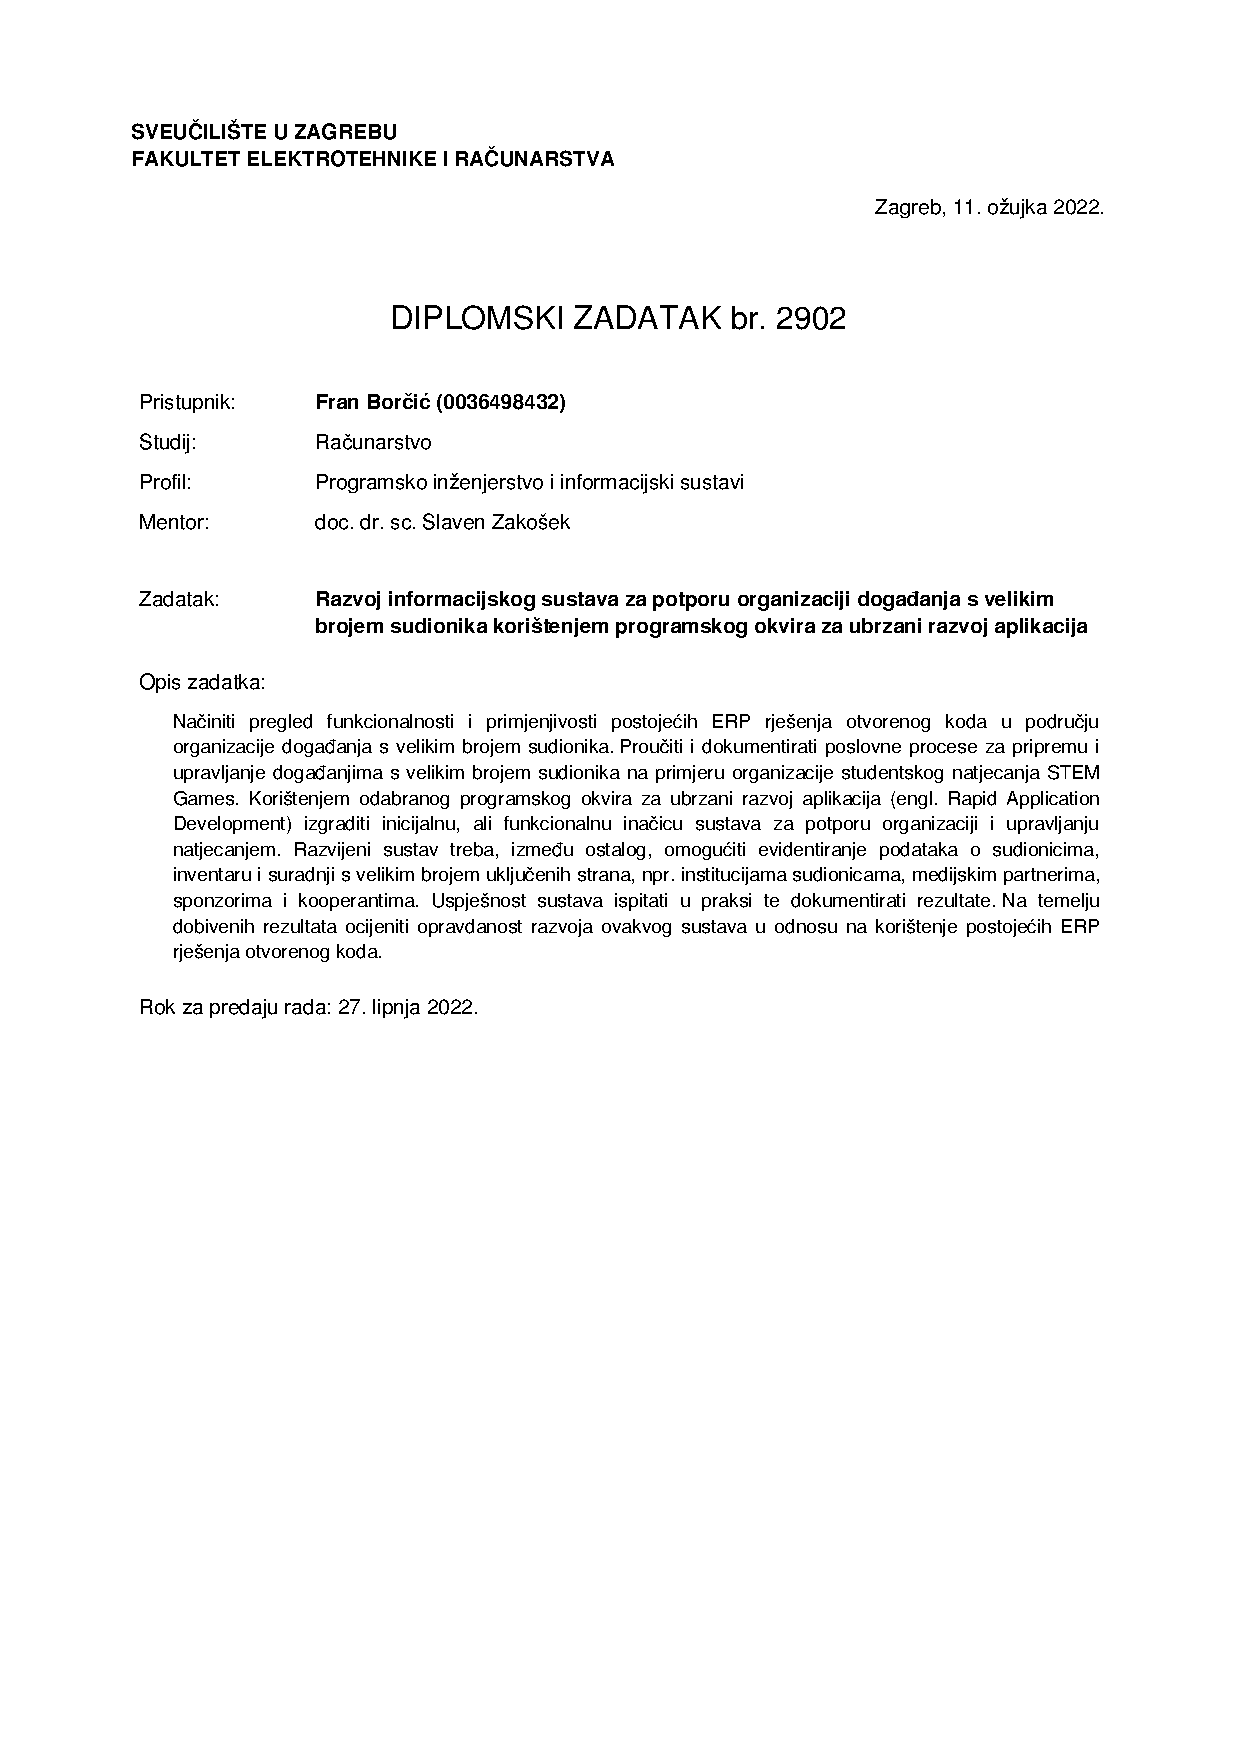
\includepdf{zadatak.pdf}

% \zahvala{}

\tableofcontents

\chapter{Uvod}

Cilj ovog rada je ocijeniti mogućnost i isplativost implementacije
informacijskog sustava u rad studentskih organizacija koje se bave organizacijom
studentskih natjecanja s velikim brojem sudionika. Problemu će se pristupiti s
dva različita aspekta -- analizom prikladnosti postojećih rješenja i razvojem
osnovnog, ali primjenjivog prilagođenog rješenja koristeći programski okvir za
ubrzani razvoj aplikacija \engl{RAD}, a vodeći se konkretnim primjerom
\emph{Udruge za studentska natjecanja STEM Games}.

Tijekom posljednjih nekoliko desetljeća svjedočimo sve većoj prisutnosti
informacijskih sustava u poslovanju komercijalnih organizacija, većinom u vidu
radnih okvira poznatih kao \emph{ERP} sustavi. Pojam \emph{ERP rješenje}
\engl{enterprise resource planning} obuhvaća veliki broj informacijskih sustava
različitih vrsta i primjena, no prema definicijama navedenima u
(\cite{evolutionerp})
taj se pojam odnosi na sustave koje karakterizira modularnost te centralizirana
pohrana svih podataka vezanih uz poslovanje jedne organizacije.

Većina takvih sustava danas je realizirana kao skup gotovih modula oblikovanih
prema generičkim potrebama većeg broja komercijalnih organizacija
(\cite{bradford2014modern}). S obzirom na broj poslovnih procesa prisutnih u
svakoj takvoj organizaciji, takva arhitektura omogućuje ubrzanu implementaciju
većeg dijela informacijskog sustava i ponovnu uporabu novorazvijenih modula u
organizacijama sličnog područja rada.

Logična je posljedica spomenute arhitekture da je uvođenje ERP sustava u
poslovanje to jeftinije i jednostavnije što je više poslovnih procesa organizacije
u koju se uvodi prisutno i u drugim organizacijama. Organizacije koje se bave
rijetkim i specifičnim zadacima ograničene su u broju dostupnih rješenja kojima
mogu digitalizirati svoje poslovanje pa je slijedom toga i isplativost njihove
informatizacije znatno manja.

Slučaj koji će u ovom radu biti proučen, osim zbog svojih poslovnih procesa,
specifičan je i prema svojim ciljevima -- organizacija studentskih natjecanja na
području RH tradicionalno je neprofitnog karaktera, a iza takvih događaja stoje
studentske udruge ili udruge građana čiji su članovi volonteri. Iz tog razloga,
potencijalni benefiti uvođenja informacijskog sustava u tom području očitovali
bi se prije svega u jednostavnosti obavljanja volonterskog rada, a u znatno
manjoj mjeri kroz financijske pokazatelje. Također, takve organizacije uglavnom
ne mogu u svojim budžetima opravdati profesionalnu izradu informacijskog
sustava, ali su im dostupni ljudski resursi u obliku studenata volontera.

Eventualni informacijski sustavi koji bi bili prikladni za takve organizacije,
bili bi osmišljeni tako da se studenti volonteri uz minimalnu edukaciju mogu
brinuti o uvođenju i održavanju takvih sustava. S obzirom na sličnosti u formatu
različitih studentskih natjecanja na području RH, kroz ovaj rad nastojat će se
pronaći rješenje koje bi olakšalo organizaciju svih takvih događanja, a čija
primjena bi zahtijevala što manje tehničkog znanja.

Takvo što moglo bi se postići primjenom ERP rješenja otvorenog koda i prethodnom
pripremom njihove konfiguracije za konkretni zadatak organizacije. ERP rješenja
otvorenog koda za neprofitne organizacije postoje te će biti razmotrena u
nastavku rada, no s obzirom na činjenicu da se u ovom slučaju radi o vrlo
specifičnom tipu neprofitne organizacije takva rješenja ne mogu pokriti sve
njene potrebe.

Bolje prilagođeno rješenje, ali tehnički zahtjevnije za održavanje, moglo bi se
ostvariti korištenjem programskih okvira za ubrzani razvoj aplikacija
\engl{RAD}. Takvi programski okviri automatiziraju izradu čestih elemenata
korisničkog sučelja prema vezanom podatkovnom modelu te time omogućuju brzu
izradu programske potpore čiji je glavni zadatak pohrana podataka. Fokus ovog
rada upravo je razvoj ovakvog rješenja, ocjena njegove primjenjivosti te
potencijal za primjenu u većem broju organizacija.

U poglavlju koje slijedi bit će opisane organizacijske strukture \emph{Udruge za
studentska natjecanja STEM Games} te njihovi zadaci prema podacima iz godišnjih
izvještaja različitih organizacijskih timova koji su sudjelovali na prethodnim
projektima te udruge. Ti će zadaci, odnosno poslovni procesi koje oni uključuju,
kasnije poslužiti za izolaciju zahtjeva na informacijski sustav koji bi pružao
podršku organizaciji studentskih natjecanja. Zatim će biti razmotrena dostupna
ERP rješenja otvorenog koda te broj zahtjeva koji bi se njihovom primjenom
zadovoljio, nakon ćega će biti opisano rješenje ostvareno koristeći RAD
programski okvir. Naposljetku, razvijeno rješenje bit će empirički ocijenjeno
prema iskustvima unutar spomenutog STEM Games organizacijskog tima te će se
sažeti zaključci o primjenjivosti informacijskih sustava u organizacijama tog
tipa.

\chapter{Primjer strukture organizacije}

U ovom poglavlju, na primjeru \emph{Udruge za studentska natjecanja STEM Games}
čiji je glavni projekt organizacija godišnjeg natjecanja za studente STEM
fakulteta pod imenom STEM Games, bit će opisane temeljne procedure potrebne za
organizaciju takvog događaja. Spomenuta organizacija, koju će se dalje u radu iz
praktičnih razloga zvati \emph{organizacija STEM Games}, poslužit će kao primjer
jer je autoru koji je u trenutku pisanja rada na njenom čelu dostupan veliki
broj podataka o dosadašnjim projektima udruge.

Zbog složenosti strukture organizacija ove vrste, praktičnije ju je opisati na
konkretnom primjeru organizacije koja se njome bavi. Dalje će se, međutim,
nastojati odvojiti koncepte proizašle iz opisa koji slijedi od konkretne STEM
Games organizacije, u skladu s nastojanjem da rezultati rada budu primjenjivi na
sve slične organizacije.

U svrhu lakšeg razumijevanja organizacije STEM Games, valja prvo ukratko opisati
događaj kojim se bavi.

\section{Natjecanje STEM Games}

Organizacija STEM Games nastala je i djeluje s ciljem da se studentima STEM
fakulteta omogući događanje na kojem se sudjelovanjem na natjecateljskim
aktivnostima mogu povezati s kolegama s drugih institucija te predstavnicima
industrije u njihovoj budućoj struci. Samo natjecanje osmišljeno je po modelu
već postojećih studentskih događanja u regiji, uz određene prilagodbe vezane
specifično uz STEM područje i suradnju s industrijom.

Organizacija jednom godišnje organizira natjecanje na kojem okuplja između
tisuću i dvije sudionika, odnosno petnaest do dvadeset visokoobrazovnih
institucija.  Studenti sudionici, prema kategorijama dostupnim u trenutku
pisanja ovog rada, natječu se u rješavanju problemskih zadataka STEM područja,
sportskim disciplinama ili računalnim igrama. Uz to, na prijedlog volontera
organizira se dodatni program u obliku neslužbenih natjecanja, predavanja,
koncertnih događanja i slično.

Središnji element ovog konkretnog natjecanja je tzv. \emph{natjecanje u znanju}
u kojem se timovi sudionika natječu u primjeni znanja stečenog na svojim
fakultetima. Radi se o četiri odvojena natjecanja u kojima se natječu timovi
studenata prirodoslovnog, tehnološkog, inženjerskog ili matematičkog usmjerenja,
rješavajući probleme koji se u suradnji s predstavnicima industrije modeliraju
prema problemima s kojima će se sresti na budućem radnom mjestu.  \footnote{Taj
    element omogućuje financiranje organizacije kroz sponzorsku suradnju; u
    smislu ovog rada, bitno je uzeti u obzir da je ta mogućnost specifična za
    natjecanje u STEM području i da veći broj ostalih studentskih natjecanja ne
uključuje takav program.}

Glavne zadaće organizacije STEM Games uključuju omogućavanje provedbe svih
natjecateljskih elemenata, logističko i financijsko planiranje, prikupljanje
sredstava, pronalazak volontera, komunikaciju s institucijama sudionicama i
promotivne aktivnosti.

\section{Hijerarhijska struktura organizacije}

Zbog velikog opsega događanja, u organizaciji dosadašnjih izdanja svake je
godine dosad sudjelovalo oko 150 volontera. Kako bi se organizacijski tim te
veličine uspješno koordinirao, organizacija je ustrojena hijerarhijski te dijeli
volontere u različite timove ovisno o zadatku kojim se bave.

Na slici \ref{fig:hier} prikazana je podjela organizacije po timovima čiji će
zadaci biti opisani u nastavku. Cjelokupnu organizaciju koordiniraju dva
\emph{voditelja organizacije} uz pomoć voditelja pojedinih organizacijskih
timova, u kojima je također prisutan interni ustroj. Detalji ustroja timova za
svrhe ovog rada nisu relevantni, no gruba podjela organizacije prikazana je kako
bi se u nastavku organizacijski zadaci mogli smisleno podijeliti po timovima
koji ih izvršavaju.

U potpoglavljima koja slijede po timovima će biti opisani oni njihovi zadaci u
čijoj provedbi potencijalni informacijski sustav može biti koristan.

\begin{figure}[H]
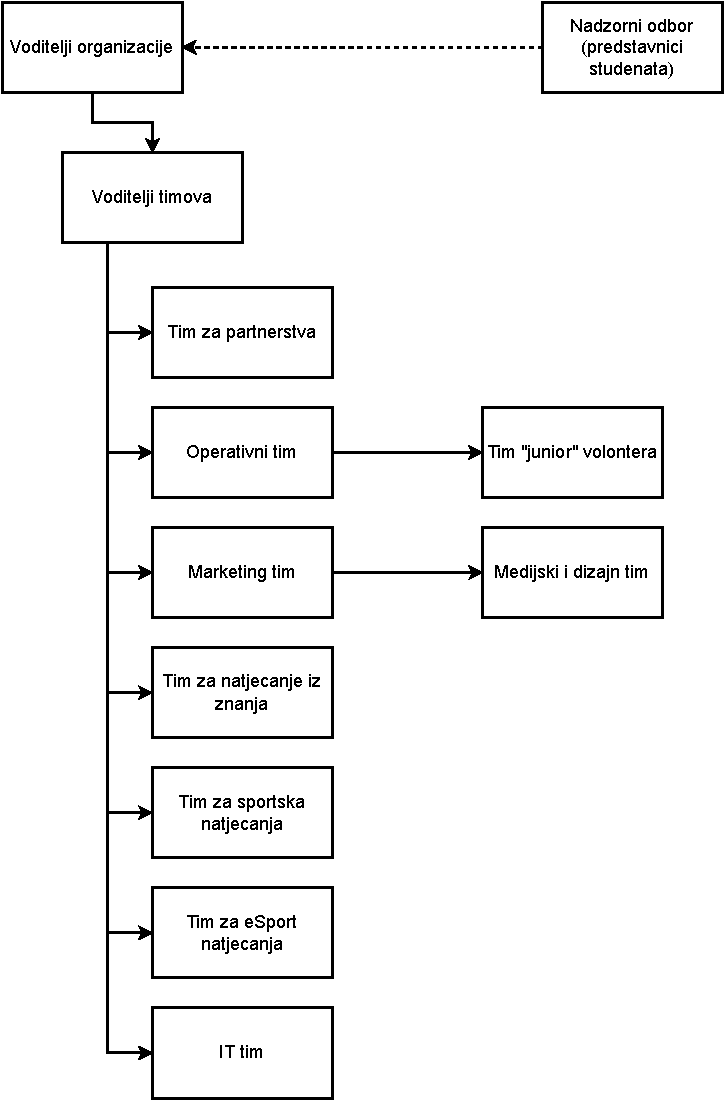
\includegraphics{slike/hijerarhija.pdf}
\caption{Prikaz organizacijskog ustroja}
\label{fig:hier}
\end{figure}

\section{Zadaci voditelja organizacije}
Voditelji organizacije, za koje su predviđene dvije pozicije u organizacijskoj
strukturi, započinju organizaciju projekta početkom akademske godine. Zaduženi
su, najprije, za okupljanje predstavnika studenata institucija koje će
sudjelovati.

Predstavnici onih institucija koje su dosad sudjelovale na natjecanju čine tzv.
\emph{nadzorni odbor} koji potvrđuje voditelje organizacije za tu godinu.
Voditelji organizacije potom digitalnim putem objavljuju natječaj za volontere u
organizaciji, od kojih se biraju drugi članovi organizacije uz potvrdu nadzornog
odbora.

Nakon ustroja organizacijskog tima, voditelji organizacije zaduženi su za
vremensko i resursno planiranje organizacije. Moraju voditi računa o
potencijalnim izvorima financiranja i rashodima potrebnima za organizaciju,
konzultirati nadzorni odbor o željama sudionika te ih uzeti u obzir prilikom
planiranja zadataka za organizacijske timove. Također, brinu se o suradnji s
kooperantom koji omogućuje prostor u kojem će se odvijati natjecanje te
posreduju u komunikaciji između ugostitelja i predstavnika institucija
sudionica.

Osim toga, voditelji organizacije brinu se o neprofitnoj organizaciji koja stoji
iza organizacijskog tima natjecanja. Brinu se o ispravnom bilježenju prihoda i
rashoda u suradnji s računovodstvenim servisom, ugovorima sa sponzorima i
kooperantima, održavanju skupština udruge i općenitim administrativnim poslovima
koji su za nju vezani.

\section{Zadaci studentskih predstavnika}

Studentski predstavnici posreduju u komunikaciji između organizacijskog tima i
studenata visokoobrazovnih institucija koje sudjeluju na natjecanju. Prema
prethodnom sudjelovanju, neki od predstavnika studenata imaju pravo glasati o
pitanjima vezanim uz tijek organizacije. To čine digitalnim putem ili na
sastancima nadzornog odbora koje sazivaju voditelji organizacije.

Predstavnici također biraju studente koje će njihova institucija povesti na
natjecanje nakon što se studenti prijave preko jedinstvene stranice
organizacije. Zaduženi su i za organizaciju prijevoza sudionika na događaj te
eventualnog sufinanciranja njihovog sudjelovanja fakultetskim ili sponzorskim
subvencijama.

\section{Zadaci operativnog tima}

Operativni tim kao organizacijski tim u užem smislu ima veliki broj zadaća, te
je možda više od bilo kojeg drugog tima podložan informatizaciji. Glavne zadaće
operativnog tima su briga o nabavi, upravljanje inventarom, organizacija
lokalnog prijevoza, upravljanje timom "junior" volontera\footnote{volontera koji
    ne sudjeluju u organizaciji, ali pomažu fizički u provedbi samog događaja},
    organizacija dodatnog programa, akreditacija sudionika te briga o rasporedu
    događanja.

Detaljni zahtjevi na informacijski sustav od strane ovog tima, kao i drugih
timova, bit će opisani u nastavku, no ovdje vrijedi nešto detaljnije opisati
pojedinosti nabrojanih zadaća.

\subsection{Nabava i upravljanje inventarom}
Operativni tim vodi evidenciju o svim kooperantima s kojima je ostvarena
komunikacija tijekom tekućeg i prijašnjih projekata te prema tome ostvaruje
suradnje nužne za provedbu događaja. Ostali timovi iskazuju svoje potrebe za
nabavom materijala operativnom timu te članovi operativnog tima komuniciraju s
potencijalnim dobavljačima i dogovaraju nabavu. Nabavu u skladu s definiranim
budžetom odobravaju voditelji organizacije.

Veliki dio nabave potrebne za projekt odnosi se na tiskane materijale, koji se
tijekom događaja koriste za promociju sponzora i informiranje sudionika.
Prilikom nabave tiskanih materijala operativni tim mora, osim s dobavljačima,
komunicirati s \emph{timom za partnerstva} koji se brine o odobrenju materijala u
kojima se spominju sponzori događaja te \emph{medijskim i dizajn timom} koji
priprema grafičke pripreme.

Tijekom događaja, tim upravlja svim inventarom koji se koristi za provedbu
natjecanja. Brine o vlasništvu inventarskih stavki (one mogu biti posuđene, u
vlasništvu udruge, volontera ili ugostitelja), zaduženjima i ovlastima među
volonterima te lokacijama na kojima se pojedini predmeti u svakom trenutku
nalaze. Također brinu o prijevozu tih predmeta na lokaciju i njihovom povratku
vlasnicima.

\subsection{Lokalni prijevoz i prijevoz organizacije}

Jedan od zadataka operativnog tima također je osigurati prijevoz članova
organizacijskog tima na mjesto događaja. Pritom mora voditi računa o lokaciji
polaska različitih članova organizacije i rasporedu njihovog dolaska po danima.

Na lokaciji natjecanja mora brinuti o zaduženjima službenih vozila u najmu i
prioritetima za njihovo korištenje. Također, mora koordinirati autobusni
prijevoz sudionika u različitim komponentama natjecanja do sportskih dvorana ili
dvorana u kojima se odvija natjecanje u znanju.

\subsection{Upravljanje sudionicima}

Operativni tim zadužen je također za provedbu prijava sudionika preko web
sučelja na stranicama organizacije, komunicirajući pritom s predstavnicima
studenata o njihovim procedurama selekcije i kategorijama za koje žele otvoriti
prijave. Nakon selekcija provedenih od strane matičnih institucija sudionika,
operativni tim brine o njihovim osobnim podacima, izdaje ulaznice za događaj,
brine o njihovom dolasku i odlasku te posreduje u komunikaciji s ugostiteljskom
tvrtkom.

\subsection{Dodatni program, raspored i dodatni volonteri}

Uz glavni program natjecanja, na događanju STEM Games organizira se i dodatni
program u obliku neslužbenih natjecanja, predavanja i slično. Koordinacija tog
programa u smislu rasporeda, materijalnih i ljudskih resursa također je zadatak
operativnog tima.

Na samom događaju, osim članova organizacijskog tima, organizaciji pomažu i
volonteri u smislu fizičke i logističke potpore. Operativni tim zadužen je i za
vodstvo spomenutog tima volontera od kojih je svaki dužan utrošiti unaprijed
određeni broj sati dnevno na dodijeljena zaduženja. Jedna od zadaća volonterskog
tima je i prihvat sudionika na dolasku, pri čemu je brzina obrade pristiglog
sudionika vrlo važna i u čemu im informacijski sustav može pomoći.

\section{Zadaci tima za partnerstva}

Glavna zadaća partnerskog tima je omogućiti organizaciju događaja prikupljanjem
sredstava od sponzora u industriji. Zadaće ovog tima posebno su podložne
informatizaciji jer je za njihovo uspješno obavljanje potrebno pomno bilježiti
svu dosadašnju komunikaciju vezanu za ostvarene i potencijalne suradnje.

Organizacija sponzorima nudi uslugu promocije kroz izlaganje i distribuciju
promotivnih materijala te uključivanje u osmišljanje problemskog dijela
natjecanja. Te su usluge definirane kroz sponzorske pakete, koji ujedno
predstavljaju i moguće kategorije sponzora.

Rezultati rada partnerskog tima u obliku ugovora o suradnji sa sponzorima usko
su vezani uz financijske elemente organizacije te bi se stoga ta veza trebala
moći pratiti u potencijalnom dijelu informacijskog sustava vezanom uz
financijsko planiranje.

% TODO: dodati neku referencu za CRM
\section{Zadaci tima za marketing i komunikacije te podtimova}

Tim za marketing i komunikacije zadužen je za pružanje informacija o događaju
široj javnosti te njegovu promociju. Pritom se koristi web stranicom, profilima
na društvenim mrežama te medijskim partnerstvima. Svojim radom pruža vidljivost
kako samom događaju, tako i sponzorskim institucijama koje omogućuju financijska
sredstva za provedbu događaja. Pod taj tim također spadaju i timovi za grafički
dizajn i fotografiju koji se brinu za kreiranje materijala potrebnih za
promociju događaja.

S aspekta informatizacije, potrebe ovog tima svode se na praćenje ostvarenih i
potencijalnih kontakata s medijskim partnerima, katalogizaciju fotografskih i
video materijala te planiranje objava na kanalima digitalne komunikacije.

\section{Timovi za natjecanja u sportu, znanju i računalnim igrama}

Timovi za natjecanja bave se organizacijom sportskih i problemskih natjecanja te
natjecanja u računalnim igrama. Njihovi zadaci tiču se sastavljanja rasporeda,
zadataka za natjecatelje ili pripreme sportskih terena. Veći dio zadataka tih
timova nije relevantan za razvoj informacijskog sustava, pa time ne spada u
okvire ovog rada.

\section{Ostale potrebe}

Važan aspekt organizacijske strukture, a koji je zajednički svim timovima tiče
se upravljanja pravima pristupa. Iako se ne radi o konkretnom organizacijskom
zadatku, u svrhu potpunosti ovog opisa kao podloge za izolaciju zahtjeva, valja
navesti problematiku.

Navedeni se timovi u svom radu koriste raznim internetskim servisima. Neki od
tih servisa omogućuju individualnu registraciju korisnika, no kod nekih se
korisnički podaci za prijavu dijele među više osoba.

Posljedica te prakse je da se osjetljivi podaci dijele u kanalima koji za to
nisu predviđeni što uzrokuje sigurnosne rizike i poteškoće u praćenju korisnika
koji u nekom trenutku imaju pristup usluzi.

Informacijski bi sustav u ovom aspektu mogao omogućiti sigurno dijeljenje
pristupnih podataka prema potrebama i ovlastima članova organizacijskog tima. U
slučaju promjene osoba u ulogama ovlaštenim za pristup nekom servisu, zaporke bi
se mogle jednostavnije promijeniti jer bi sustav omogućio da se o toj promjeni
jednostavno obavijeste svi članovi tima koji koriste određeni servis.

Drugi aspekt kontrole pristupa je onaj fizički. Na samom događaju, uspostavljaju
se organizacijski ured i skladište kojemu mogu pristupiti samo određeni članovi
organizacije. Informatizacijom ovog aspekta pristup prostorima mogao bi se
kontrolirati digitalnim putem, korištenjem uređaja već ustaljenih za tu namjenu
poput RFID sustava, što bi otvorilo prostor za povećanu sigurnost u odnosu na
korištenje tradicionalnih metoda poput korištenja papirnatih akreditacija.

\chapter{Podaci organizacije za pohranu u IS}

Nastavno na prethodni opis organizacije, a u svrhu ocjene prikladnosti ERP
sustava otvorenog koda i kasnijeg razvoja prilagođenog rješenja, valja
definirati potrebe organizacije koje bi informacijski sustav u primjeni trebao
zadovoljavati.

S obzirom na prirodu organizacijskih potreba, funkcionalni zahtjevi svode se na
pohranu podataka različite vrste u sistematiziranom formatu, dok za njihovom
obradom nema izražene potrebe. Slijedom toga, u aplikaciji se ne zahtjeva sloj
poslovne logike, te će se funkcionalni zahtjevi proučavati s aspekta podataka
koje aplikacija mora pohranjivati. Implicitno će se podrazumjevati da aplikacija
kroz svoje sučelje mora ponuditi operacije upisa, čitanja, modifikacije te
brisanja \engl{CRUD}, te da se prema pravilima organizacijske strukture za svaki
od definiranih podatkovnih entiteta može upravljati ovlastima kategorija
korisnika kojima je te operacije dopušteno izvoditi.

U ovom će poglavlju u svrhu analize zahtjeva opisno biti prikazane kategorije
podataka koje organizacija mora moći pohraniti u sustavu te njihovi međusobni
odnosi. Kako se od gotovih rješenja ne može očekivati podudarnost s potrebama
organizacije u idealnom slučaju, prije njihove ocjene njihove prikladnosti neće
se ulaziti u konkretne strukture podatkovnog modela, već će zahtjevi biti
razmotreni na višoj razini. Razrada i formalizacija konkretnog relacijskog
modela odgodit će se za poglavlje o rješenju korištenjem RAD programskog okvira.

\section{Podaci o osobama}

Organizacija natjecanja ovog tipa zahtjeva pohranu osobnih podataka velikog
broja različitih kategorija osoba povezanih s događajem. Imajući u vidu
osjetljivu prirodu osobnih podataka, vrlo je korisno omogućiti njihovu pohranu
na jednom mjestu, kako s aspekta informacijske sigurnosti tako i zbog
jednostavnosti upravljanja skupom podataka.

Osobni podaci koji se pohranjuju mogu pripadati članovima organizacijskog tima,
sudionicima natjecanja ili članovima drugih organizacija s kojima se surađuje
tijekom organizacije natjecanja. Ovisno o kategoriji pojedinca čiji se podaci
pohranjuju, tih podataka može biti više ili manje. Osnovni podaci uvijek su ime
i prezime osobe, kontakt podatak koji može biti adresa elektroničke pošte ili
broj telefona te pripadnost organizacijama i institucijama. Ovisno o potrebi,
tome se može nadodati datum rođenja, adresa stanovanja, neka vrsta jedinstvenog
identifikacijskog broja te u konkretnom slučaju opisane organizacije i veličina
majice, u svrhu izrade promotivnih materijala.

Uz osobne podatke, moraju se pratiti i podaci o sudjelovanju pojedinca na
konkretnom događaju. Ti će podaci biti opisani kasnije, ovisno o kategoriji
sudjelovanja osobe u pitanju.

\section{Korisnici sustava i uloge}

Neke od osoba čiji bi se podaci bilježili u sustavu istovremeno bi bili
korisnici tog sustava. U sustavu se moraju moći definirati korisnici uz svoje
pristupne podatke te se različite korisnike mora moći povezati sa zapisima o
njihovim osobnim podacima.

Svaki korisnik mora imati definirana prava pristupa različitim podacima
pohranjenim u sustavu te prava njihove izmjene u smislu operacija upisa,
modifikacije i brisanja. Kako se prava ne bi definirala pojedinačno za svakog
korisnika, u sustavu mora postojati koncept uloge kao skupa prava koji se može
unaprijed definirati i dodijeliti korisniku ovisno o njegovim organizacijskim
potrebama i ovlastima.

Svaki korisnik može imati više uloga te svaka uloga može biti pridružena većem
broju korisnika, a prava izmjene i dodjele uloga također su jedna od ovlasti
koja može biti omogućena jednoj od uloga. Ovakav pristup sigurnosti, poznat kao
RBAC \engl{role-based access control} vrlo je raširen (\cite{rbac}), te je stoga
izgledno da gotova rješenja nude takve mogućnosti.

\section{Podaci o organizacijama i institucijama}

Osim podataka o osobama uključenim u organizaciju događaja, važno je pohraniti
podatke o raznovrsnim organizacijama i institucijama koje su važne za njegovu
provedbu. To uključuje obrazovne institucije, sponzore, medijske partnere,
kooperante te partnerske organizacije.

Većina podataka o organizaciji ovisi o prirodi angažmana te organizacije unutar
projekta, te će stoga biti pobrojani u kasnijim potpoglavljima. Jedini obavezni
podatak u zapisu o pojedinoj organizaciji je njezino ime, a dodatni
(fakultativni) podaci uključuju adresu sjedišta organizacije, njezin matični
broj, relaciju prema kontakt osobama, generički kontakt organizacije te podatke
o njezinom angažmanu na pojedinim projektima, poželjno u obliku relacije prema
odvojenom zapisu o njezinom sudjelovanju.

\section{Podaci o projektima}

Svaki projekt, odnosno događanje koje se organizira, mora se moći zabilježiti u
informacijskom sustavu uz svoje predviđene datume početka i završetka. U zapisu
projekta nema potrebe za navođenjem ostalih podataka, ali se putem relacijskih
veza moraju moći dohvatiti različiti zapisi koji se odnose na pojedini projekt.

Ti će zapisi biti nabrojani u nastavku, a uključuju dokumente, budžet, ugovore i
račune, sponzorstva, sudjelovanja osoba, kooperante i vezane podatke.

\section{Podaci o sudjelovanju obrazovne institucije}

Osnovni podaci svake obrazovne institucije koja sudjeluje na natjecanju moraju
biti zapisani u dijelu informacijskog sustava koji pohranjuje podatke o
organizacijama i institucijama, no kao odvojenu kategoriju treba pohraniti i
podatke o njihovom sudjelovanju na konkretnom projektu. Ti podaci uključuju
relaciju prema projektu na kojem sudjeluju, relaciju prema osobama koje
ispunjavaju ulogu predstavnika studenata za tu godinu, procjenu broja sudionika,
broj glasova u nadzornom odboru na koji ta institucija eventualno ima pravo,
te kategorije natjecanja u kojima želi sudjelovati.

Poželjno je da zapis o sudjelovanju obrazovne institucije bude izravno povezan
sa zapisima o sudjelovanju njenih studenata na konkretnom natjecanju na koje se
zapis o sudjelovanju odnosi.

\section{Podaci o inventaru}

Informacijski sustav mora omogućiti pohranu podataka o inventaru dostupnom
organizaciji, koji može biti u vlasništvu organizacije, privatne osobe ili
pravne treće osobe. Zapis o inventarskoj stavci, dakle, mora sadržavati ime te
stavke po kojem ju se može identificirati, jedinstveni numerički identifikator,
oznaku lokacije relaciju prema zapisu o vlasniku (osobi ili organizaciji) te
relaciju prema osobi trenutno zaduženoj za brigu o stavci.

Dodatno, treba postojati mogućnost otpisa stavke, što može provesti brisanjem
stavke ili označavanjem polja koje ukazuje na status otpisa. Koristeći tu
mogućnost, zapisi o inventaru mogu se primijeniti i za praćenje potrošne robe.

\section{Podaci o dokumentu}

Uz fizički inventar organizacije, važno je pratiti i dokumente koji su od
organizacijskog značaja. To mogu biti financijski, pravni ili organizacijski
dokumenti, a glavni atributi zapisa o njima su naslov dokumenta, autor, vrijeme
nastanka te lokacija (fizička ili virtualna) na kojoj se dokument nalazi.

Uz to, u svrhu lakšeg pretraživanja dokumenata, bilo bi korisno omogućiti upis
kratkog opisa dokumenta.

\section{Podaci o sponzoru}

Prilikom komunikacije sa sponzorskim organizatorima, bilježenje povijesti
kontakata može biti od velike pomoći partnerskom timu koji osigurava sredstva za
održavanje događaja. Stoga je u informacijskom sustavu za potporu
organizacijskom timu, potrebno omogućiti pohranu podataka o suradnji s pojedinom
sponzorskom organizacijom.

Zapis o sponzorstvu poželjno bi relacijski bio vezan uz pojedini projekt i
organizaciju, a sadržavao bi razinu interesa koju je sponzor iskazao, kratki
opis sponzora, komentare o korespondenciji te relacijsku veze prema volonteru koji
je odgovoran za komunikaciju sa sponzorom i eventualnim sklopljenim ugovorima.

Takav zapis omogućio bi detaljni uvid u povijest suradnje s pojedinim sponzorom
u bilo kojem trenutku.

% TODO: referenca na CRM
\section{Podaci o sudjelovanju natjecatelja}

Uz prijavu sudionika natjecatelja, za koju je važno imati zapis u informacijskom
sustavu, osim osobnih podataka vežu se i podaci vezani uz sudjelovanje te osobe
na pojedinom natjecanju. Ti podaci odnose se na kategorije u kojima se sudionik
natječe, identifikacijsku oznaku tima za one discipline u kojima se natječu
timovi te fakultativno smještajnu jedinicu u kojoj je sudionik smješten.

\section{Podaci o sudjelovanju volontera}

Važna organizacijska informacija jest i interni ustroj organizacije. S obzirom
na praksu da na različitim projektima ista osoba može obavljati različite uloge,
praktična funkcionalnost sustava bila bi da se za osobu koja radi na konkretnom
projektu može odrediti njezina funkcija kroz pripadnost timu.

Zbog različitih zadataka koje članovi istog tima mogu obavljati, ovaj je koncept
odvojen od uloge u smislu ovlasti korisnika sustava. Bilo bi, dakle, poželjno da
sustav omogućuje pohranu zapisa o pripadnosti pojedine osobe projektnim timovima
te povezivanje tog zapisa sa zapisom o izravno nadređenom volonteru ako takav
postoji.

\section{Podaci o računima}

Iako se o knjigovodstvu organizacije brinu za to stručni kooperanti, zbog
interne evidencije sustav treba omogućiti osnovno praćenje izlaznih i ulaznih
faktura. Izlazne fakture uvijek su vezane uz sponzore, a ulazne fakture uz
kooperante. Uz to, svaka je faktura dokument, te bi zapisi o fakturama morali
biti vezani uz pripadajuće zapise o dokumentima.

Svaki zapis o fakturi trebao bi sadržavati fakturirani iznos, datum izdavanja,
datum dospjeća i podatak o tome je li plaćanje izvršeno. Dodatno, zapisi o
izlaznim fakturama trebali bi sadržavati broj pod kojim je faktura izdana.

\section{Podaci o vozilima}

Tijekom provedbe samog natjecanja, organizacija mora voditi evidenciju o
korištenju vozila koje uzima u najam. Stoga bi bilo korisno omogućiti praćenje
planiranih i obavljenih vožnji vezanih uz pojedino vozilo.

Sustav bi u tu svrhu morao omogućiti upisivanje zapisa o vozilu te povezivanje
tog zapisa sa zapisima o rezervacijama vozila za planirane vožnje kao i zapisima
o obavljenim vožnjama. Svaki zapis o vožnji morao bi biti vezan uz osobu vozača,
polazište i odredište te vrijeme polaska i povratka.

Koristan dodatak zapisima o vožnjama bio bi podatak o stanju spremnika za gorivo
kako bi se za to zaduženim osobama omogućilo da na vrijeme opskrbe vozilo
gorivom.

\section{Podaci o budžetu}

Uz svaki projekt, veže se i plan raspodjele očekivanih sredstava. Sustav mora
omogućiti rudimentarno financijsko planiranje u obliku zapisa o kategoriji
troška te njegovom iznosu. Poželjna nadogradnja bila bi da se ulazne fakture
mogu povezati s nekim od zapisa u spomenutom planu, odnosno pojedinom budžetskom
stavkom.

\section{Podaci o kooperantima}

Na isti način kako partnerski tim bilježi podatke o sponzorima, operativni tim
trebao bi moći zabilježiti podatke o kooperantima. Zapis o kooperantu uključivao
bi komentare o prethodnoj suradnji, relacijsku vezu s relevantnim zapisom o
organizaciji te projektom na kojem se odvija suradnja te veze sa svim ulaznim
fakturama izdanim od strane spomenutog kooperanta.

\section{Pristupni podaci za mrežne usluge}

Sustav bi također trebao omogućiti siguran prostor za pohranu pristupnih
podataka vezanih uz korisničke račune na internetskim servisima koje koristi
više osoba unutar organizacijskog tima. Svaki zapis o korisničkom računu mora
sadržavati ime servisa kojem se pristupa, korisničko ime i zaporku, a
relacijskom vezom mora biti ustanovljeno koje sve korisničke uloge imaju pravo
pročitati pojedini zapis.

Sustav mora ograničiti pristup ovim podacima samo na one uloge koje su za
korištenje tih podataka ovlaštene te lozinke mora pohranjivati u kriptografski
zaštićenom formatu.

\section{Podaci o medijskom partneru}

Naposljetku, sustav mora omogućiti praćenje kontakata i korespondencije s
medijskim partnerima događaja. Zahtjevi za ovu evidenciju identični su onima za
evidenciju sponzorstava, no s obzirom na to da se odnosima s medijima bavi drugi
tim, te dvije kategorije moraju biti razdvojene.

Dodatno, bilo bi poželjno omogućuiti povezivanje medijskog partnera s medijskim
objavama koje su mu predložene. Zapis medijske objave tada bi trebao povezivati
zapis o dokumentu koji je izvorno izdao i poslao organizacijski tim, zapis o
medijskom partnerstvu te, ukoliko postoji, poveznicu na objavu od strane medija.

\chapter{Dostupni \emph{ERP} sustavi otvorenog koda}
\chapter{Rješenje primjenom \emph{RAD} programskog okvira}

\chapter{Zaključak}
...
\bibliography{literatura}
\bibliographystyle{fer}

\begin{sazetak}
Sažetak na hrvatskom jeziku.

\kljucnerijeci{Ključne riječi, odvojene zarezima.}
\end{sazetak}

% TODO: Navedite naslov na engleskom jeziku.
\engtitle{Title}
\begin{abstract}
Abstract.

\keywords{Keywords.}
\end{abstract}

\end{document}
